\section{RGB laserový modul}
Jako zdroj laserového paprsku byl~využit RGB~laserový modul, skládající se~ze~řídící desky, tří barevných laserových diod o~vlnových délkách 660~nm~(červená), 450~nm~(modrá) a~520~nm~(zelená) a~tří dichroických zrcátek, která slouží ke~spojení paprsků z~diod do~jednoho. Celý modul je~vidět na~obrázku~\ref{fig:hw_laser-module}.


\begin{figure}[htb]
  \centering
  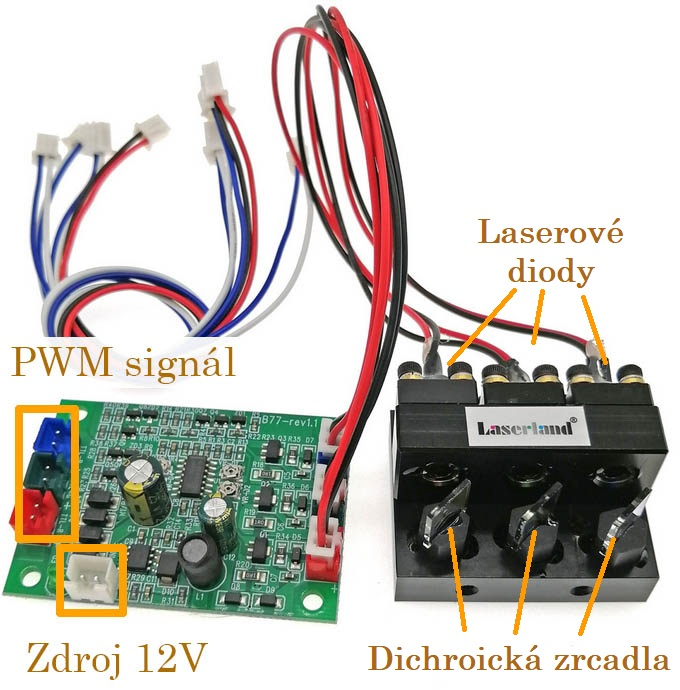
\includegraphics[width=0.6\textwidth]{img/hw_laser-module.jpg}
  \caption{\label{fig:hw_laser-module} Laserový modul s~řídící deskou a~vyznačenými konektory}
\end{figure}

\subsection{Dichroická zrcadla}

Dichroická zrcadla jsou zrcadla s~výrazně rodílnými odrazovými nebo průchodovými vlastnostmi pro~dvě různé vlnové délky odraženého/procházejícího světla~\cite{dichroic-mirrors}.

Většina dichroických zrcadel jsou dielektrická zrcadla, která se~skládají z~mnoha tenkých vrstev různě opticky propustných materiálů. Existují ale~také krystalická zrcadla, jejiž odrážlivá vrstva se~skládá z~monokrystalického materiálu, typicky polovodiče~\cite{dichroic-mirrors}.

Mezi jejich využití spadá například oddělování infračerveného záření při aplikacích, kdy~je~nežádoucí zahřívání ozařovaného objektu~\cite{dichroic-mirrors}.

\subsection{Zapojení laserového modulu}
K modulu je~od~výroby připojená řídící deska. Ta~požaduje napětí 12 ~V~a~přijímá binární signál pro~každou diodu. Je-li na~signál připojena zem, korespondující dioda nesvítí. Je-li na~něj připojeno 2,7 až 5~V, korespondující dioda svítí.

\subsection{Tvorba barev s~laserovým modulem}
S laserem je~tedy možné vytvořit 7 barev -- červenou, zelenou, modrou, žlutou, tyrkysovou, purpurovou a~bílou, viz~obrázek~\ref{fig:7colors}.

\begin{figure}[htb]
  \centering
  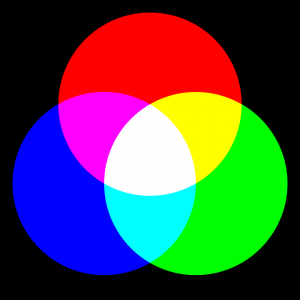
\includegraphics[width=0.3\textwidth]{img/7colors.png}
  \caption{\label{fig:7colors} Sedm základních barev laserového modulu}
\end{figure}

Naštěstí i ~zde~je~možné uplatnit jev~persistance of~vision a~sice pomocí techniky PWM~popsané v~kapitole~\ref{sec:pwm}.
Nastavíme-li tedy střídu signálu pro~červenou diodu na~100~\% a ~pro~zelenou diodu na~50~\% výsledný paprsek bude pro~lidské oko~mít barvu s~rgb hodnotou (255, 127, 0) neboli oranžovou.

I tato technologie má ovšem své limitace, řídící deska laserového modulu zvládá přijímat signál o~maximální frekvenci 35 ~kHz~(Raspberry Pi~je~schopno vysílat s~frekvencí až 40~kHz), což vzhledem k~rychlosti pohybu laseru v~některých případech nemusí stačit.
Může se~stát, že při vykreslování křivky se~paprsek stihne posunout dříve, než uplyne perioda pwm~signálu. Pokud se ~tak~stane, budou různé sousední části křivky mít různou barvu.

\fxnote{TODO obrázek nedostatečně rychleho pwm}

Tento efekt je~nejviditelnější při projekci tmavých barev, ale~dá se~zmírnit zvětšením času, po~který paprsek setrvá na~jednom bodě po~jeho vykreslení, v~tu~chvíli se ~ale~může stát, že nastane \uv{flickering} popsaný v~sekci~\ref{sec:projection-princip}.